% Options for packages loaded elsewhere
% Options for packages loaded elsewhere
\PassOptionsToPackage{unicode}{hyperref}
\PassOptionsToPackage{hyphens}{url}
\PassOptionsToPackage{dvipsnames,svgnames,x11names}{xcolor}
%
\documentclass[
  indonesian,
  letterpaper,
  DIV=11,
  numbers=noendperiod]{scrreprt}
\usepackage{xcolor}
\usepackage[margin=1in]{geometry}
\usepackage{amsmath,amssymb}
\setcounter{secnumdepth}{5}
\usepackage{iftex}
\ifPDFTeX
  \usepackage[T1]{fontenc}
  \usepackage[utf8]{inputenc}
  \usepackage{textcomp} % provide euro and other symbols
\else % if luatex or xetex
  \usepackage{unicode-math} % this also loads fontspec
  \defaultfontfeatures{Scale=MatchLowercase}
  \defaultfontfeatures[\rmfamily]{Ligatures=TeX,Scale=1}
\fi
\usepackage{lmodern}
\ifPDFTeX\else
  % xetex/luatex font selection
\fi
% Use upquote if available, for straight quotes in verbatim environments
\IfFileExists{upquote.sty}{\usepackage{upquote}}{}
\IfFileExists{microtype.sty}{% use microtype if available
  \usepackage[]{microtype}
  \UseMicrotypeSet[protrusion]{basicmath} % disable protrusion for tt fonts
}{}
\makeatletter
\@ifundefined{KOMAClassName}{% if non-KOMA class
  \IfFileExists{parskip.sty}{%
    \usepackage{parskip}
  }{% else
    \setlength{\parindent}{0pt}
    \setlength{\parskip}{6pt plus 2pt minus 1pt}}
}{% if KOMA class
  \KOMAoptions{parskip=half}}
\makeatother
% Make \paragraph and \subparagraph free-standing
\makeatletter
\ifx\paragraph\undefined\else
  \let\oldparagraph\paragraph
  \renewcommand{\paragraph}{
    \@ifstar
      \xxxParagraphStar
      \xxxParagraphNoStar
  }
  \newcommand{\xxxParagraphStar}[1]{\oldparagraph*{#1}\mbox{}}
  \newcommand{\xxxParagraphNoStar}[1]{\oldparagraph{#1}\mbox{}}
\fi
\ifx\subparagraph\undefined\else
  \let\oldsubparagraph\subparagraph
  \renewcommand{\subparagraph}{
    \@ifstar
      \xxxSubParagraphStar
      \xxxSubParagraphNoStar
  }
  \newcommand{\xxxSubParagraphStar}[1]{\oldsubparagraph*{#1}\mbox{}}
  \newcommand{\xxxSubParagraphNoStar}[1]{\oldsubparagraph{#1}\mbox{}}
\fi
\makeatother


\usepackage{longtable,booktabs,array}
\usepackage{calc} % for calculating minipage widths
% Correct order of tables after \paragraph or \subparagraph
\usepackage{etoolbox}
\makeatletter
\patchcmd\longtable{\par}{\if@noskipsec\mbox{}\fi\par}{}{}
\makeatother
% Allow footnotes in longtable head/foot
\IfFileExists{footnotehyper.sty}{\usepackage{footnotehyper}}{\usepackage{footnote}}
\makesavenoteenv{longtable}
\usepackage{graphicx}
\makeatletter
\newsavebox\pandoc@box
\newcommand*\pandocbounded[1]{% scales image to fit in text height/width
  \sbox\pandoc@box{#1}%
  \Gscale@div\@tempa{\textheight}{\dimexpr\ht\pandoc@box+\dp\pandoc@box\relax}%
  \Gscale@div\@tempb{\linewidth}{\wd\pandoc@box}%
  \ifdim\@tempb\p@<\@tempa\p@\let\@tempa\@tempb\fi% select the smaller of both
  \ifdim\@tempa\p@<\p@\scalebox{\@tempa}{\usebox\pandoc@box}%
  \else\usebox{\pandoc@box}%
  \fi%
}
% Set default figure placement to htbp
\def\fps@figure{htbp}
\makeatother



\ifLuaTeX
\usepackage[bidi=basic,provide=*]{babel}
\else
\usepackage[bidi=default,provide=*]{babel}
\fi
% get rid of language-specific shorthands (see #6817):
\let\LanguageShortHands\languageshorthands
\def\languageshorthands#1{}


\setlength{\emergencystretch}{3em} % prevent overfull lines

\providecommand{\tightlist}{%
  \setlength{\itemsep}{0pt}\setlength{\parskip}{0pt}}



 


% Warna judul agar mirip contoh (beige keemasan halus)
\usepackage{xcolor}
\definecolor{titleaccent}{RGB}{183,176,138} % #b7b08a

% Paket yang diperlukan
\usepackage{pdfpages}   % untuk menyisipkan cover.pdf
\usepackage{graphicx}   % untuk cover berbentuk gambar (opsional)

% Nonaktifkan title bawaan Pandoc (\maketitle) agar tidak dobel
\makeatletter
\AtBeginDocument{\let\maketitle\relax}
\makeatother
\KOMAoption{captions}{tableheading}
\makeatletter
\@ifpackageloaded{bookmark}{}{\usepackage{bookmark}}
\makeatother
\makeatletter
\@ifpackageloaded{caption}{}{\usepackage{caption}}
\AtBeginDocument{%
\ifdefined\contentsname
  \renewcommand*\contentsname{Daftar Isi}
\else
  \newcommand\contentsname{Daftar Isi}
\fi
\ifdefined\listfigurename
  \renewcommand*\listfigurename{Daftar Gambar}
\else
  \newcommand\listfigurename{Daftar Gambar}
\fi
\ifdefined\listtablename
  \renewcommand*\listtablename{Daftar Tabel}
\else
  \newcommand\listtablename{Daftar Tabel}
\fi
\ifdefined\figurename
  \renewcommand*\figurename{Gambar}
\else
  \newcommand\figurename{Gambar}
\fi
\ifdefined\tablename
  \renewcommand*\tablename{Tabel}
\else
  \newcommand\tablename{Tabel}
\fi
}
\@ifpackageloaded{float}{}{\usepackage{float}}
\floatstyle{ruled}
\@ifundefined{c@chapter}{\newfloat{codelisting}{h}{lop}}{\newfloat{codelisting}{h}{lop}[chapter]}
\floatname{codelisting}{Daftar}
\newcommand*\listoflistings{\listof{codelisting}{Daftar Daftar}}
\makeatother
\makeatletter
\makeatother
\makeatletter
\@ifpackageloaded{caption}{}{\usepackage{caption}}
\@ifpackageloaded{subcaption}{}{\usepackage{subcaption}}
\makeatother
\usepackage{bookmark}
\IfFileExists{xurl.sty}{\usepackage{xurl}}{} % add URL line breaks if available
\urlstyle{same}
\hypersetup{
  pdflang={id},
  colorlinks=true,
  linkcolor={blue},
  filecolor={Maroon},
  citecolor={Blue},
  urlcolor={Blue},
  pdfcreator={LaTeX via pandoc}}


\author{}
\date{}
\begin{document}

% (opsional) gunakan penomoran romawi untuk front matter
\pagenumbering{roman}

% --- COVER ---
% Jika Anda punya cover.pdf (1 halaman)
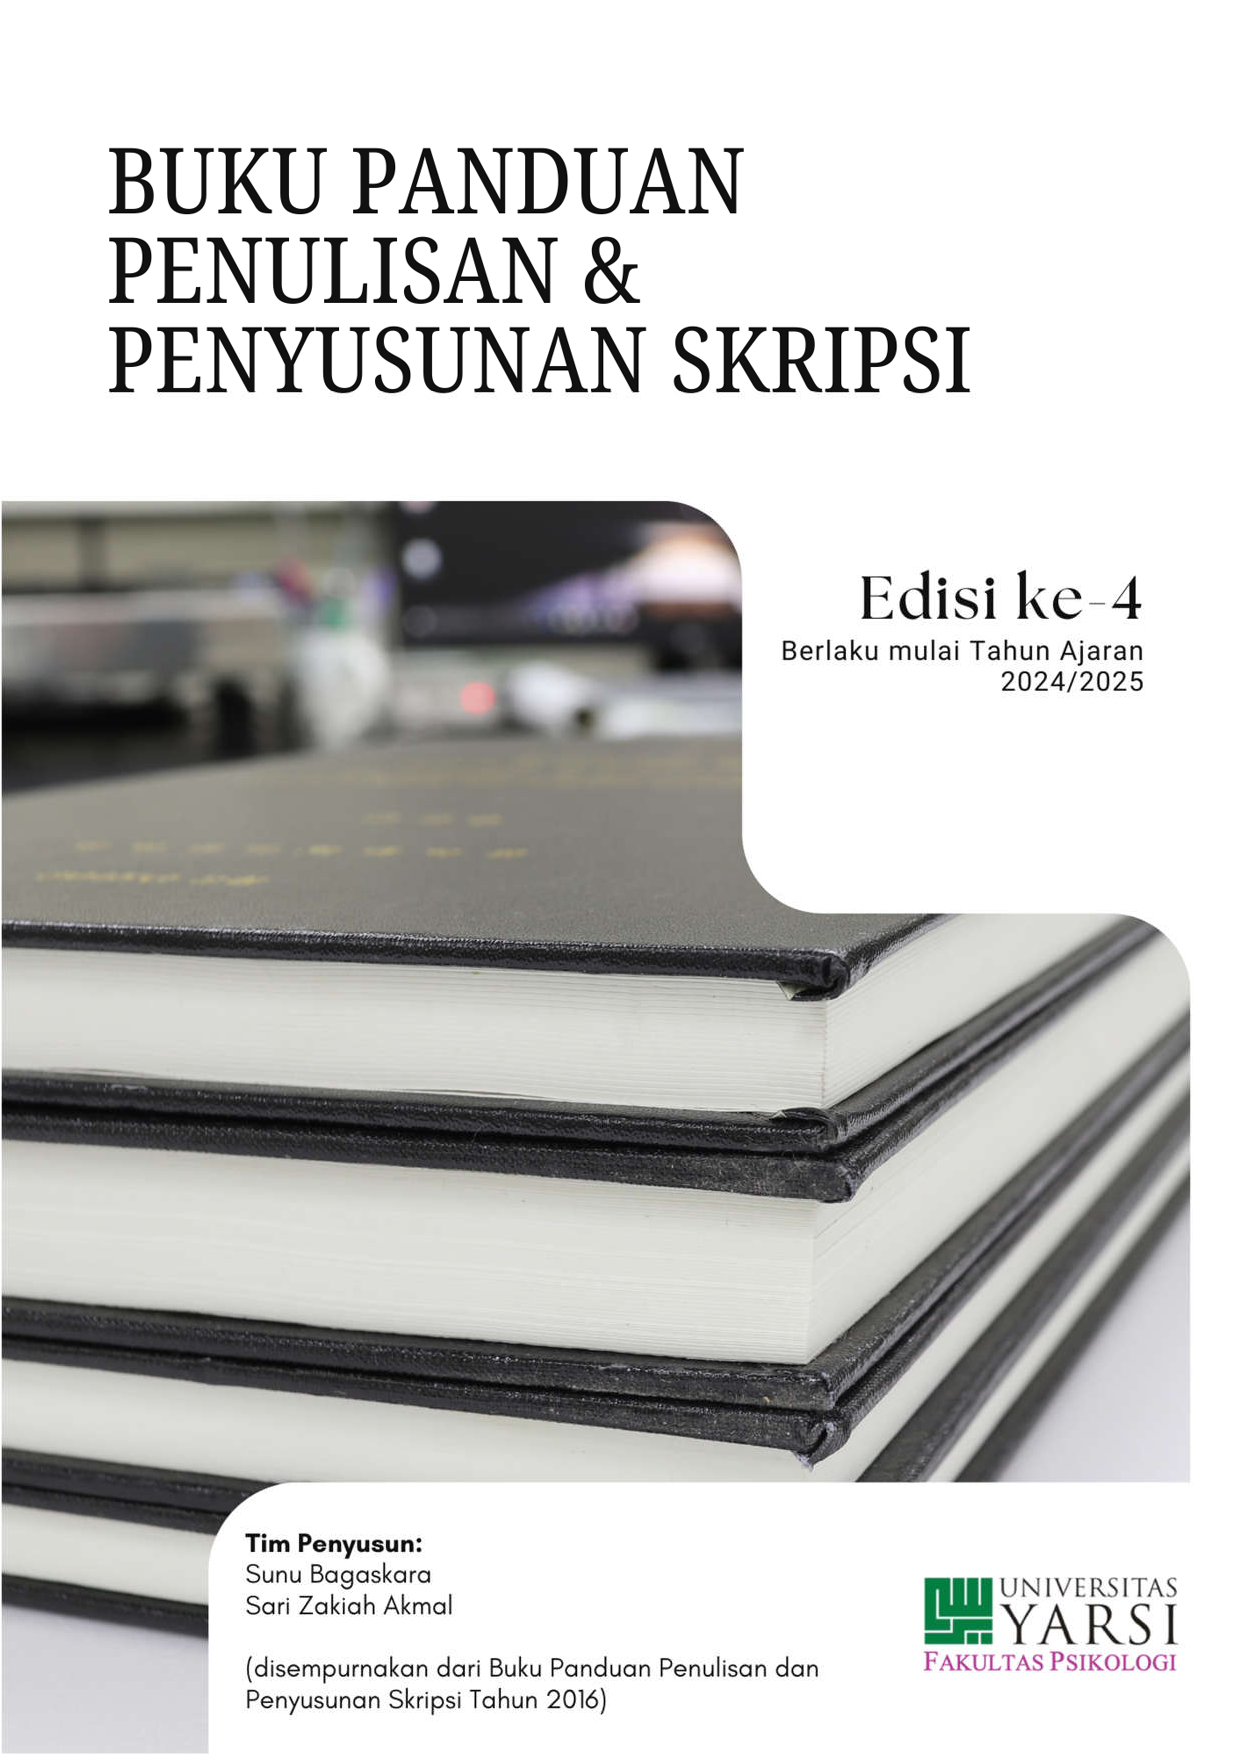
\includepdf[pages=1,fitpaper=true]{cover.pdf}
\cleardoublepage

% --- HALAMAN JUDUL ---
\begin{titlepage}
\centering
\vspace*{2.5cm}
{\fontsize{22pt}{26pt}\selectfont\bfseries Buku Panduan\\[2mm]}
{\fontsize{22pt}{26pt}\selectfont\bfseries Penulisan \& Penyusunan Skripsi\par}

\vspace{1.2cm}
\rule{\linewidth}{0.5pt}\\[-6pt]
{\large \textbf{Fakultas Psikologi Universitas YARSI}}\par
\rule{\linewidth}{0.5pt}

\vspace{1.4cm}
{\large \textbf{Edisi Ke-4}\par}

\vfill
{\large \textbf{Tim Penyusun:}}\par
{\large Sunu Bagaskara\par}
{\large Sari Zakiah Akmal\par}
\vspace*{1.2cm}
\end{titlepage}
\cleardoublepage

% --- BALIK HALAMAN JUDUL (verso) ---
\thispagestyle{empty}
\vspace*{\fill}
\begin{center}
\textit{Buku Panduan Penulisan \& Penyusunan Skripsi}\\
Fakultas Psikologi Universitas YARSI\\[6pt]
Hak Cipta © 2025 Fakultas Psikologi Universitas YARSI\\
ISBN: (isi bila ada)
\end{center}
\vspace*{\fill}
\clearpage

\renewcommand*\contentsname{Daftar Isi}
{
\hypersetup{linkcolor=}
\setcounter{tocdepth}{2}
\tableofcontents
}

\bookmarksetup{startatroot}

\chapter*{\texorpdfstring{\textbf{Pendahuluan}}{Pendahuluan}}\label{pendahuluan}
\addcontentsline{toc}{chapter}{\textbf{Pendahuluan}}

\markboth{\textbf{Pendahuluan}}{\textbf{Pendahuluan}}

Dalam perjalanan akademis, penulisan skripsi merupakan salah satu fase
krusial yang harus dilalui oleh setiap mahasiswa di perguruan tinggi.
Skripsi tidak hanya berfungsi sebagai salah satu syarat untuk mencapai
gelar akademik, tetapi juga sebagai bukti kemampuan mahasiswa dalam
melakukan penelitian yang sistematis dan mendalam terhadap suatu
masalah. Melalui skripsi, mahasiswa ditantang untuk menerapkan
pengetahuan yang telah mereka peroleh selama perkuliahan, sekaligus
mengembangkan kemampuan analisis, kritis, dan ilmiah mereka.

Tujuan dari buku ini adalah untuk memberikan panduan praktis dan teknis
dalam menulis skripsi. Buku ini dirancang untuk membantu mahasiswa dalam
merencanakan, melakukan dan menyajikan hasil penelitian mereka dalam
bentuk skripsi yang sistematis dan logis. Melalui panduan ini, mahasiswa
diharapkan dapat memahami langkah-langkah penulisan skripsi, mulai dari
pemilihan topik yang relevan, penyusunan proposal penelitian,
pengumpulan dan analisis data, hingga penyajian hasil penelitian dan
kesimpulan.

Penggunaan buku ini disarankan untuk dijadikan sebagai acuan atau
pedoman selama proses penulisan skripsi. Buku ini disusun dengan bahasa
yang mudah dipahami dan disertai dengan contoh serta tips praktis yang
akan sangat membantu dalam memecahkan berbagai kendala yang sering
dihadapi mahasiswa selama proses penulisan skripsi. Di awal buku,
pembaca akan dibawa untuk memahami konsep-konsep dasar skripsi dan
perbedaannya dengan karya ilmiah lainnya. Kemudian, dilanjutkan dengan
pembahasan secara mendetil mengenai posisi skripsi dalam kurikulum
Fakultas Psikologi Universitas YARSI. Pembahasannya meliputi persyaratan
serta prosedur teknis pendaftaran ujian skripsi.

Setelah membahas konsep dasar dan posisi skripsi dalam kurikulum, buku
ini akan memandu pembaca menyelami prinsip-prinsip penting yang harus
dikuasai mahasiswa untuk memulai petualangannya dalam menulis skripsi.
Salah satu kunci sukses dalam penulisan skripsi adalah pemilihan topik.
Topik yang dipilih tidak hanya harus sesuai dengan minat dan keahlian
mahasiswa, tetapi juga relevan dengan bidang ilmu pengetahuan yang
sedang dikaji. Topik yang baik adalah topik yang dapat memberikan
kontribusi bagi pengembangan ilmu pengetahuan, sekaligus mampu menjawab
masalah aktual yang ada di masyarakat. Dalam buku ini, pembaca akan
diajak untuk memahami berbagai pertimbangan dalam memilih topik skripsi,
serta strategi dalam mengembangkan ide penelitian menjadi sebuah
proposal penelitian yang solid dan meyakinkan.

Selanjutnya, buku ini juga akan membahas secara sekilas mengenai teknik
pengumpulan data, baik kualitatif maupun kuantitatif, serta cara-cara
untuk menganalisis data tersebut. Mahasiswa akan diajarkan bagaimana
cara menginterpretasikan hasil penelitian dan menyajikannya dalam bentuk
narasi ilmiah yang koheren dan logis. Selain itu, aspek penting lainnya
seperti penulisan daftar pustaka, pengutipan sumber, dan penyusunan
lampiran juga akan dibahas untuk memastikan bahwa skripsi yang
dihasilkan tidak hanya berkualitas tinggi dari segi konten, tetapi juga
memenuhi standar akademik yang berlaku.

Dengan memahami isi dari buku ini, diharapkan mahasiswa dapat menavigasi
proses penulisan skripsi dengan lebih mudah dan efisien, serta pada
akhirnya dapat menghasilkan skripsi yang tidak hanya memenuhi standar
akademik, tetapi juga dapat menjadi kontribusi yang berarti bagi
pengembangan ilmu pengetahuan dan masyarakat.

Tim Penulis,

Juni 2024

Tim Penulis,

Agustus 2024

\bookmarksetup{startatroot}

\chapter*{Pengenalan Skripsi}\label{pengenalan-skripsi}
\addcontentsline{toc}{chapter}{Pengenalan Skripsi}

\markboth{Pengenalan Skripsi}{Pengenalan Skripsi}

Skripsi merupakan sebuah karya tulis ilmiah yang disusun oleh mahasiswa
sebagai salah satu syarat untuk memperoleh gelar sarjana. Skripsi tidak
hanya merefleksikan kemampuan akademik mahasiswa, tetapi juga kemampuan
mereka dalam menerapkan teori ke dalam praktik penelitian yang konkret.
Dalam proses pembelajaran di perguruan tinggi, penulisan skripsi
berperan penting dalam pengembangan keterampilan penelitian, kritis, dan
analitis mahasiswa. Menurut Sugiyono (2018), skripsi merupakan
penelitian ilmiah yang sistematis dan mendalam pada suatu fenomena atau
masalah dengan tujuan mengembangkan dan menguji teori-teori yang ada
dalam disiplin ilmu tertentu.

\section*{1.1 Tujuan Skripsi}\label{tujuan-skripsi}
\addcontentsline{toc}{section}{1.1 Tujuan Skripsi}

\markright{1.1 Tujuan Skripsi}

Tujuan utama dari penulisan skripsi adalah untuk menunjukkan bahwa
mahasiswa mampu melakukan penelitian yang independen, sistematis, dan
ilmiah. Selain itu, skripsi juga bertujuan untuk menguji kemampuan
mahasiswa dalam menyusun argumen yang logis, mengelola dan menganalisis
data, dan menyajikan hasil penelitian secara tertulis yang memenuhi
standar akademik. Menurut Creswell (2014), melalui skripsi, mahasiswa
diharapkan dapat mengidentifikasi masalah penelitian, merumuskan
hipotesis, mengumpulkan dan menganalisis data, serta menyimpulkan dan
merekomendasikan solusi terhadap masalah yang diteliti.

\section*{1.2 Perbedaan Skripsi, Tesis, dan
Disertasi}\label{perbedaan-skripsi-tesis-dan-disertasi}
\addcontentsline{toc}{section}{1.2 Perbedaan Skripsi, Tesis, dan
Disertasi}

\markright{1.2 Perbedaan Skripsi, Tesis, dan Disertasi}

Penting untuk memahami perbedaan antara skripsi, tesis, dan disertasi,
karena ketiganya merupakan karya tulis ilmiah yang berbeda, terutama
dalam hal tujuan, kedalaman analisis, dan tingkat pendidikan. Skripsi
ditulis oleh mahasiswa sarjana sebagai bagian dari proses penyelesaian
studi mereka. Tesis merupakan karya tulis ilmiah yang disusun oleh
mahasiswa pascasarjana (magister) dan lebih kompleks serta mendalam
dibandingkan skripsi. Disertasi adalah karya ilmiah yang disusun oleh
mahasiswa doktoral dan merupakan kontribusi original terhadap
pengetahuan yang ada, membutuhkan penelitian yang lebih komprehensif dan
mendalam. Kumar (2014) menjelaskan bahwa tingkat kedalaman dan kebaruan
penelitian meningkat secara signifikan dari skripsi ke tesis dan dari
tesis ke disertasi.

\section*{1.3 Proses Penulisan Skripsi}\label{proses-penulisan-skripsi}
\addcontentsline{toc}{section}{1.3 Proses Penulisan Skripsi}

\markright{1.3 Proses Penulisan Skripsi}

Proses penulisan skripsi umumnya melibatkan beberapa tahap, mulai dari
pemilihan topik, penyusunan proposal, pengumpulan data, analisis data,
hingga penulisan laporan skripsi. Proses ini membutuhkan waktu,
dedikasi, dan upaya yang signifikan dari mahasiswa. Bazeley (2013)
menekankan pentingnya manajemen waktu dan organisasi yang baik dalam
proses penulisan skripsi untuk memastikan bahwa mahasiswa dapat
menyelesaikan skripsinya dengan efisien dan efektif.

Pemilihan topik skripsi yang tepat sangat krusial karena akan menentukan
arah dan fokus penelitian. Mahasiswa disarankan untuk memilih topik yang
tidak hanya sesuai dengan minat dan keahlian mereka, tetapi juga relevan
dengan kebutuhan masyarakat atau bidang ilmu pengetahuan. Setelah topik
dipilih, mahasiswa harus menyusun proposal penelitian yang mencakup
latar belakang masalah, tujuan penelitian, metodologi, dan rencana
kerja. Proposal ini nantinya akan diuji dan disetujui oleh dosen
pembimbing sebelum penelitian dapat dimulai.

Pengumpulan data merupakan tahap penting dalam penulisan skripsi, dimana
mahasiswa harus menggunakan metodologi yang sesuai untuk mengumpulkan
data yang relevan dengan masalah penelitian. Metode pengumpulan data
dapat berupa kualitatif, kuantitatif, atau kombinasi dari kedua metode
tersebut. Setelah data terkumpul, mahasiswa kemudian menganalisis data
tersebut untuk mengidentifikasi pola, hubungan, atau temuan penting yang
dapat menjawab pertanyaan penelitian.

Penulisan laporan skripsi merupakan tahap akhir dari proses penulisan
skripsi. Laporan ini harus menyajikan hasil penelitian secara jelas,
logis, dan sistematis, serta memenuhi standar penulisan ilmiah. Laporan
skripsi umumnya terdiri dari beberapa bab, termasuk pendahuluan,
tinjauan pustaka, metodologi penelitian, hasil dan pembahasan, serta
kesimpulan dan saran.

\section*{Kesimpulan}\label{kesimpulan}
\addcontentsline{toc}{section}{Kesimpulan}

\markright{Kesimpulan}

Skripsi adalah sebuah proses penelitian ilmiah yang membutuhkan
dedikasi, disiplin, dan kemampuan analitis yang tinggi dari mahasiswa.
Melalui penulisan skripsi, mahasiswa diharapkan dapat mengembangkan
kemampuan penelitian mereka dan memberikan kontribusi terhadap
pengembangan ilmu pengetahuan. Dengan pemahaman yang baik tentang
tujuan, perbedaan dengan tesis dan disertasi, serta proses penulisan
skripsi, mahasiswa dapat menavigasi tantangan ini dengan lebih baik dan
mencapai kesuksesan dalam penelitian mereka.




\end{document}
